\documentclass{standalone}
\usepackage{tikz}
\usepackage{amsmath}
\usetikzlibrary{matrix,chains,positioning,decorations.pathreplacing,arrows}
\usetikzlibrary{positioning, calc, chains}
\usetikzlibrary{decorations.pathreplacing}
\begin{document}


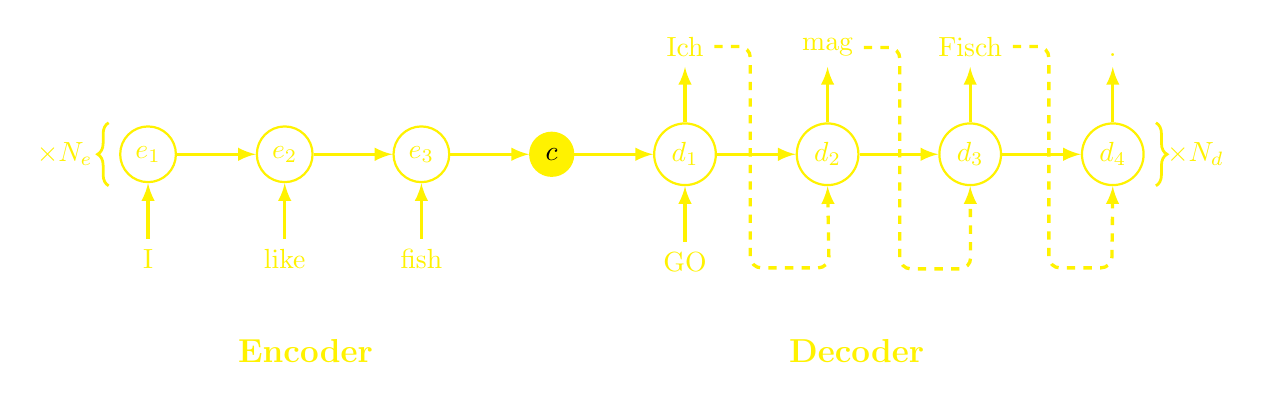
\begin{tikzpicture}[draw=yellow, item/.style={circle,draw,thick,align=center},
itemc/.style={item,on chain,join}]

%encoder
\begin{scope}[start chain=going right,nodes=itemc,every
join/.style={-latex,very thick},local bounding box=chain, xshift=-7cm]
\path 
	node[color=yellow] (e1) {$e_1$} 
	node[color=yellow] (e2) {$e_2$} 
	node[color=yellow] (e3) {$e_3$} 
	node[color=yellow, fill=yellow] (c)  {\textcolor{black}{$c$}} 
	node[color=yellow] (d1) {$d_1$} 
	node[color=yellow] (d2) {$d_2$} 
	node[color=yellow] (d3) {$d_3$} 
	node[color=yellow] (d4) {$d_4$};
\end{scope}

\draw[very thick,latex-] (e1.south) -- ++ (0,-2em)
node[below, color=yellow] {I};

\draw[very thick,latex-] (e2.south) -- ++ (0,-2em)
node[below, color=yellow] {like};

\draw[very thick,latex-] (e3.south) -- ++ (0,-2em)
node[below, color=yellow] {fish};

% context vector



% decoder input
\draw[very thick,latex-] (d1.south) -- ++ (0,-2em)
node[below, color=yellow] (i1) {GO};




% decoder output
\draw[very thick, -latex] (d1.north) -- ++ (0, 2em)
node[above, color=yellow] (o1) {Ich};

\draw[very thick, -latex] (d2.north) -- ++ (0, 2em)
node[above, color=yellow] (o2) {mag};

\draw[very thick, -latex] (d3.north) -- ++ (0, 2em)
node[above, color=yellow] (o3) {Fisch};

\draw[very thick, -latex] (d4.north) -- ++ (0, 2em)
node[above, color=yellow] (o4) {.};

% recursions
\draw[very thick,-latex, rounded corners, dashed] (o1.east) -- ++ (1.3em,0em)  -- ++ (0, -8em) -- ++ (1., 0) -- (d2.south);

\draw[very thick,-latex, rounded corners, dashed] (o2.east) -- ++ (1.3em,0em)  -- ++ (0, -8em) -- ++ (.9, 0) -- (d3.south);

\draw[very thick,-latex, rounded corners, dashed] (o3.east) -- ++ (1.3em,0em)  -- ++ (0, -8em) -- ++ (.8, 0) -- (d4.south);

%braces
\draw [decorate,decoration={brace,amplitude=4pt}, line width=1.pt] 
(-7.5,-.4) -- (-7.5,.4) node [left, midway, color=yellow, xshift=-2pt] {$\times N_e$};
\draw [decorate,decoration={brace,mirror,amplitude=4pt}, line width=1.pt]
(5.8,-.4) -- (5.8,.4) node [right, midway, color=yellow, xshift=0.2pt] {$\times N_d$};

% captions
\node at (-5,-2.5) {\textcolor{yellow}{\large \textbf{Encoder}}};
\node at (2,-2.5) {\textcolor{yellow}{\large \textbf{Decoder}}};
\end{tikzpicture}



\end{document}